\documentclass[11pt,a4paper]{article}

\usepackage[utf8]{inputenc}
\usepackage[T1]{fontenc}
\usepackage{lmodern}
\usepackage[french]{babel}
\usepackage[margin=2.1cm]{geometry}
\usepackage{microtype}
\usepackage{booktabs}
\usepackage{array}
\usepackage{amsmath}
\usepackage[table]{xcolor}
\usepackage{graphicx}
\usepackage{caption}
\usepackage[most]{tcolorbox}

\definecolor{navy}{HTML}{1F3864}
\definecolor{lightblue}{HTML}{D6E0F0}
\definecolor{accent}{HTML}{C0491F}

\captionsetup{font=small,labelfont={bf,color=navy},labelsep=period}
\graphicspath{{../../../vasicek_lab/figures/}}

\newtcolorbox{cle}[1][]{colback=lightblue!40,colframe=navy,boxrule=0.6pt,
  arc=2pt,left=8pt,right=8pt,top=6pt,bottom=6pt,#1}

\title{\vspace{-1.3cm}\color{navy}\bfseries L'identifiabilité de la contagion dirigée $W$\\[2pt]
  \large Une limite démontrée, muée en spécification de donnée}
\author{Kélian Kaddouri}
\date{\today}

\begin{document}
\maketitle
\vspace{-0.7cm}

\begin{cle}
\textbf{Thèse du chapitre.} La matrice de contagion dirigée $W$ entre les cinq piliers DORA
\emph{n'est pas identifiable} sur les données publiques disponibles. Ce n'est pas un aveu,
c'est un résultat : je le démontre sur deux sources qui échouent pour des raisons
\textbf{opposées}, je distingue proprement ce que la donnée fixe de ce qu'elle ne fixe pas
(identification \emph{partielle}), et j'en tire une \textbf{spécification de reporting}
qui, seule, rendrait $W$ estimable. La contagion reste donc un objet \textbf{normatif},
élicité et borné par la sensibilité, jamais présenté comme calibré.
\end{cle}

\section*{1. Ce qu'identifier $W$ exigerait}

Le coefficient $W_{jk}$ mesure la propension d'une défaillance du pilier $k$ à
\emph{entraîner}, dans la foulée, une défaillance du pilier $j$. L'identifier sur données
demande trois choses simultanément : (i) observer des \textbf{co-occurrences} de
défaillances de piliers au sein d'une même entité ; (ii) disposer d'une \textbf{antériorité
temporelle} fiable (qui précède qui) pour distinguer $W_{jk}$ de $W_{kj}$ ; (iii) une
\textbf{taxonomie par pilier} (domaine de contrôle), et non par vecteur d'attaque. Aucune
des deux sources examinées ne réunit les trois.

\section*{2. Deux échecs opposés}

\paragraph{Source 1 : Data Breach Chronology (notifications d'États américains).}
La base est volumineuse ($74\,783$ incidents, $25\,009$ organisations) mais inexploitable
pour $W$, par \textbf{manque de taxonomie et de volume informatif}. La catégorie
non déterminée (\texttt{UNKN}) pèse \textbf{52,7\,\%} des incidents et n'est attribuable à
aucun pilier. La date de \emph{survenance} n'est exploitable que dans \textbf{49,6\,\%} des
cas, et son caractère manquant n'est pas aléatoire : il varie par type d'incident, si bien
qu'ordonner par survenance élimine des catégories entières du panel. Ordonner par
\emph{déclaration}, l'autre date disponible, ne mesure pas la contagion mais le
\textbf{délai de détection} (qui varie d'un facteur important selon le type). Résultat : une
fois restreint aux types informatifs et aux trimestres consécutifs, il ne reste que
\textbf{71 transitions} $k(t\!-\!1)\to j(t)$ (soit $3{,}6$ observations par cellule
hors-diagonale), et \textbf{34} dans le seul secteur financier. La direction n'y est pas
estimable, faute de matière.

\paragraph{Source 2 : SAS OpRisk Global Data (pertes opérationnelles, Bâle).}
Ici le \textbf{volume est au rendez-vous} : \textbf{4\,329 transitions} annuelles entre les
7 catégories de risque, soit environ \textbf{103 observations par cellule}. Et pourtant la
direction reste inidentifiable, pour la raison \emph{opposée} : le pas de temps est
l'\textbf{année}, trop grossier pour porter une antériorité. Un test placebo le montre sans
appel. On permute les années \emph{à l'intérieur de chaque firme} (ce qui détruit toute
antériorité mais conserve la co-occurrence), et l'on recalcule l'asymétrie
$\lVert M - M^\top\rVert_1/2$ de la matrice de transition :
\[
\text{asymétrie réelle} = 119 \qquad\text{contre placebo} = 128 \pm 27
\qquad\Rightarrow\qquad z = -0{,}33 .
\]
L'asymétrie observée est \emph{sous} le bruit du placebo : aucun signal directionnel. Le
test binomial par paire confirme : sur 18 paires suffisamment peuplées, \textbf{aucune}
n'est significative à 5\,\%, ni avant ni après correction de Bonferroni. La matrice de
transition est \textbf{symétrique} : le pas annuel a lessivé la direction.

\begin{cle}
\textbf{Précaution de méthode (à afficher).} Le test intuitif du \og temps inversé \fg{}
(comparer $M$ à la matrice obtenue en renversant la chronologie) est \textbf{dégénéré} sur
un comptage : par construction $M_{\text{inv}} = M^\top$, donc la corrélation des asymétries
vaut $-1$ quel que soit le contenu. Il ne prouve rien. Seul le \textbf{placebo par
permutation} est valide sur des comptages. Le signaler est un gage de rigueur, pas une
faiblesse.
\end{cle}

\begin{center}
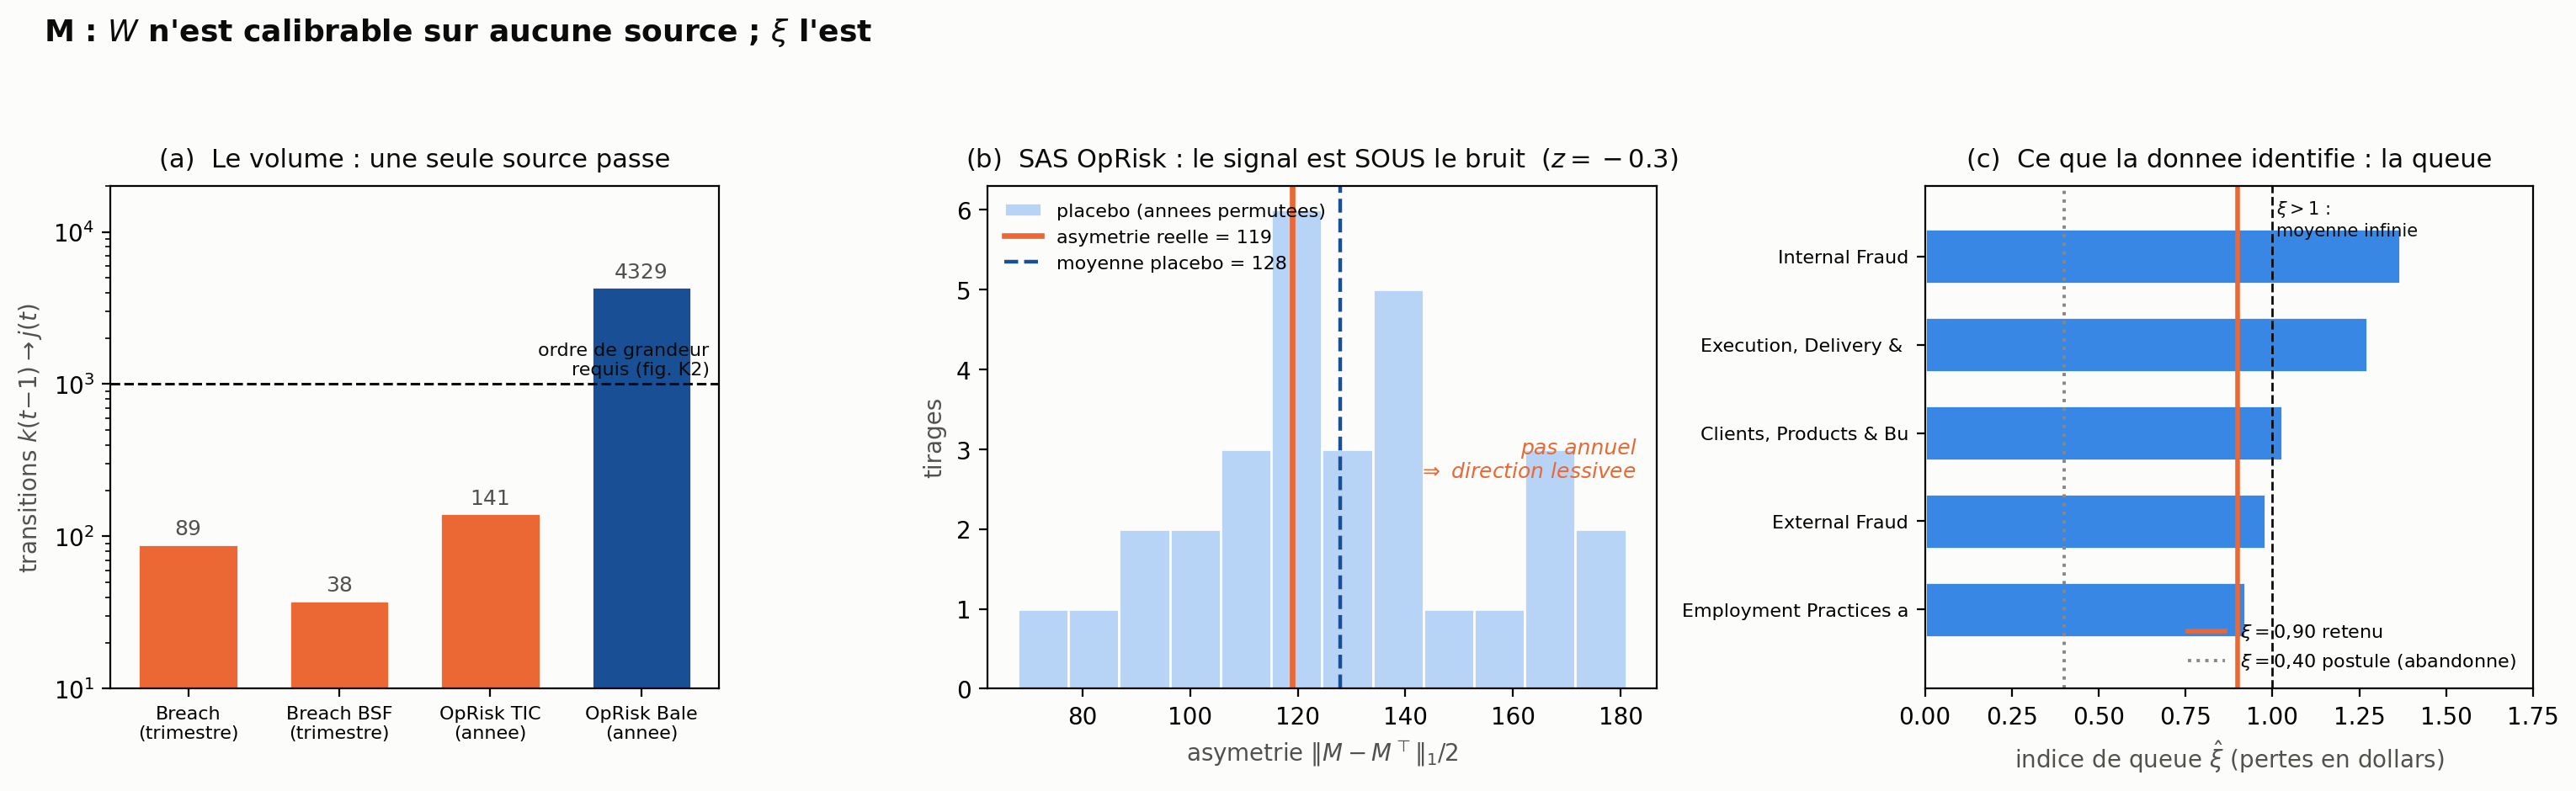
\includegraphics[width=\linewidth]{M_faisabilite.png}
\captionof{figure}{Les deux échecs et ce qui subsiste. (a)~Une seule source atteint le
volume requis. (b)~Sur cette source, le signal directionnel est sous le bruit du placebo
($z=-0{,}33$). (c)~Ce que la donnée identifie, elle : l'indice de queue $\xi$.}
\end{center}

\section*{3. Identification partielle : la frontière explicite}

L'échec n'est pas total, et c'est ce qui fait la valeur du modèle. La donnée
\textbf{fixe} plusieurs objets, qui sont ceux des chapitres empiriques :
\begin{itemize}\itemsep2pt
\item la \textbf{fréquence marginale} d'entrée (mélange de Poisson calibré) ;
\item l'\textbf{accumulation} par cause commune (concentration journalière, Gini $0{,}69$) ;
\item l'\textbf{indice de queue} de sévérité $\xi \approx 0{,}90$, avec sa sensibilité au
      seuil ($0{,}93$, $0{,}83$, $0{,}68$ aux seuils $q_{90}$, $q_{95}$, $q_{99}$) et son
      \textbf{hétérogénéité par catégorie} ($0{,}92$ à $1{,}37$ selon la catégorie Bâle),
      qui justifie un $\xi_j$ \emph{par pilier}.
\end{itemize}
Elle \textbf{ne fixe pas} la \textbf{direction hors-diagonale} de $W$. La frontière
d'identification est donc nette : les marges sont ancrées, la structure dirigée ne l'est
pas. $W$ relève alors d'un autre régime de connaissance, le \textbf{jugement d'expert
structuré} (élicitation de Cooke, chapitre suivant), et son influence est \textbf{bornée
par une analyse de sensibilité}, jamais posée comme mesurée.

\section*{4. La donnée manquante comme livrable}

Puisque les deux sources échouent pour des raisons opposées (l'une manque de volume et de
taxonomie, l'autre de résolution temporelle), la donnée qui identifierait $W$ se déduit par
complémentarité. Un registre d'incidents TIC \textbf{identifiant} $W$ devrait :
\begin{enumerate}\itemsep2pt
\item horodater la \textbf{survenance} (et non la seule déclaration) au \textbf{mois ou à la
      semaine}, afin de porter une antériorité que le pas annuel efface ;
\item catégoriser par \textbf{domaine de contrôle} (les piliers DORA), et non par vecteur
      d'attaque, afin qu'une transition soit interprétable comme un lien $k \to j$ ;
\item consolider une \textbf{cause commune} comme \emph{un} événement à $N$ victimes, pour
      ne pas confondre un batch de déclaration avec une contagion séquentielle.
\end{enumerate}
Cette spécification n'est pas un v\oe u : elle est directement opposable au cadre de
reporting DORA, dont elle constitue une \textbf{recommandation actionnable}. La limite
d'identifiabilité devient ainsi une contribution réglementaire.

\begin{cle}
\textbf{Ce que ce chapitre apporte au mémoire.} Démontrer, chiffres à l'appui, qu'une
dépendance que tout le monde \emph{postule} n'est pas \emph{mesurable} sur les données
publiques est rare et courageux. Cela transforme une faiblesse apparente (\og je n'ai pas
calibré $W$ \fg) en trois résultats : une \textbf{frontière d'identification} explicite, une
\textbf{discipline} sur l'usage de $W$ (normatif, borné, jamais sur-vendu), et une
\textbf{spécification de reporting} qui donne au travail une portée au-delà du modèle.
\end{cle}

\end{document}
